D\section{Ekran startowy aplikacji i przygotowanie danych}
Kiedy dane zostały dostosowane do działania systemu, przystąpiono do implementacji pozostałych części rozwiązania.
Kolejnym elementem jest ekran startowy aplikacji, widoczny na rysunku \ref{fig:homescreen}. Zawiera on przyciski, które przekierowują użytkownika do odpowiednich sekcji aplikacji.

\begin{figure}[h]
    \centering
    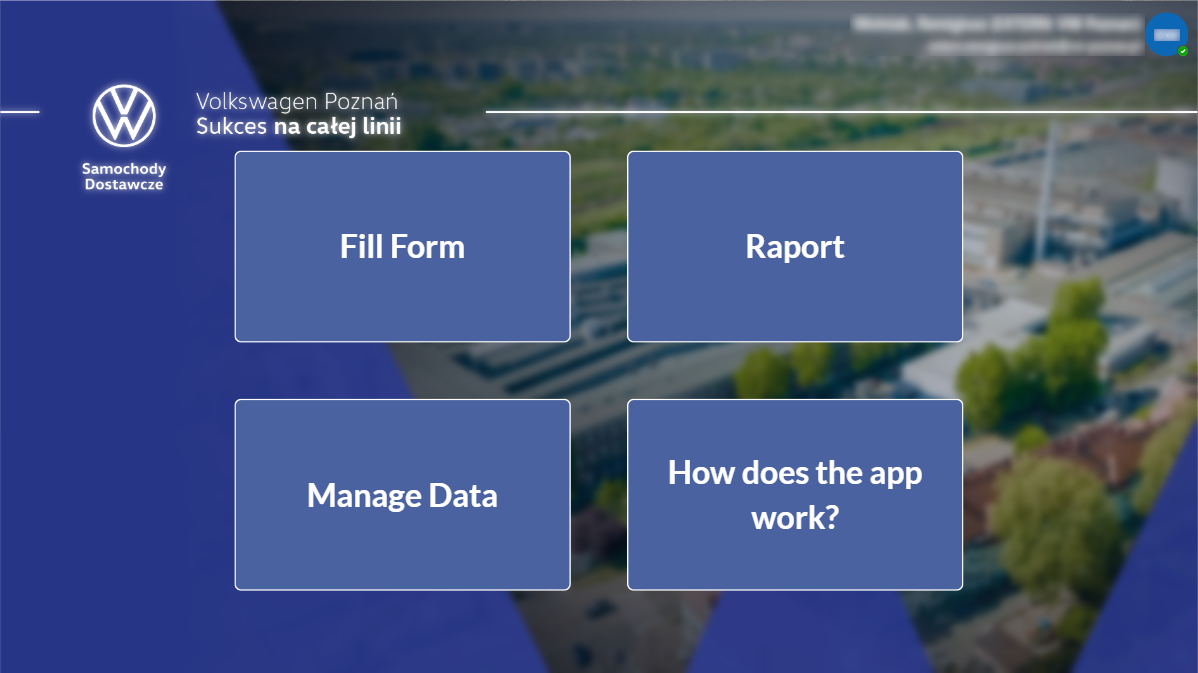
\includegraphics[width=0.9\textwidth]{figures/HomeScreen.png}
    \caption{Ekran startowy aplikacji} 
    \label{fig:homescreen}
\end{figure}

Dodatkowo, podczas uruchomienia aplikacji, pobierane są dane z list SharePointowych a następnie odpowiednio przetwarzane w celu płynnego wyświetlania ich w aplikacji. \\
Kod w języku \emph{Power Fx} wywoływany podczas uruchamiania aplikacji został przedstawiony w listingu \ref{lst:OnStartCode}.

\lstset{language=C,caption={Kod wywoływany podczas uruchamiania aplikacji},label=lst:OnStartCode}
\begin{lstlisting}[language=PowerFx]
Set(varDownloadingData; true);;
ClearCollect(colYears; 
    {Value: Text(Now(); "yyyy") - 2}; 
    {Value: Text(Now(); "yyyy") - 1}; 
    {Value: Text(Now(); "yyyy") + 0}; 
    {Value: Text(Now(); "yyyy") + 1}; 
    {Value: Text(Now(); "yyyy") + 2}
);;
Set(VWBlue; ColorValue("#002e5f"));;
ClearCollect(colNumbers; 
    {Value: 1}; 
    {Value: 2}; 
    {Value: 3}; 
    {Value: 4}; 
    {Value: 5}
);;
Set(UserVar; UżytkownicyusługiOffice365.MyProfile());;
ClearCollect(LocalServiceData; Lista_Uslug);;
ClearCollect(LocalCostData; Lista_Kwot);;
ClearCollect(LocalIndicationsData; Lista_Indykacji);;
ClearCollect(MergedData; 
    AddColumns(LocalServiceData; 
        Kwoty; LookUp(LocalCostData; 
            Service_ID = LocalServiceData[@Service_ID] && 
            Year = Max(Filter(LocalCostData; 
                Service_ID = LocalServiceData[@Service_ID]
            ); Year)
        ); 
        Indykacje; LookUp(LocalIndicationsData; 
            Service_ID = LocalServiceData[@Service_ID] && 
            Year = Max(Filter(LocalIndicationsData; 
                Service_ID = LocalServiceData[@Service_ID]
            ); Year) && 
            IndicationNo = Max(Filter(LocalIndicationsData; 
                Service_ID = LocalServiceData[@Service_ID] && 
                Year = Max(Filter(LocalIndicationsData; 
                    Service_ID = LocalServiceData[@Service_ID]
                ); Year)
            ); IndicationNo)
        )
    )
);;
Set(varDownloadingData; false);;
\end{lstlisting}

W pierwszym kroku, zmiennej \emph{varDownloadingData} przypisywana jest wartość \emph{true} za pomocą funkcji \emph{Set()}. Zmienna ta pełni kluczową rolę w zarządzaniu interfejsem użytkownika podczas procesu ładowania danych – aktywuje wskaźnik ładowania oraz blokuje możliwość wprowadzania zmian przez użytkownika, co zapobiega ewentualnym błędom wynikającym z prób modyfikacji danych w trakcie ich pobierania.

Następnie, funkcja \emph{ClearCollect()} tworzy kolekcję \emph{colYears}, która zawiera pięć elementów reprezentujących zakres lat: od dwóch lat wstecz do dwóch lat naprzód. Analogicznie, tworzona jest kolekcja \emph{colNumbers}, zawierająca numery indykacji, które mogą być wykorzystywane w polach typu \emph{Dropdown}. Kolekcje te są niezbędne do budowy dynamicznego i responsywnego interfejsu użytkownika, umożliwiając łatwe zarządzanie danymi w aplikacji.

W kolejnym kroku, za pomocą funkcji \emph{Set()}, pobierane są informacje o aktualnie zalogowanym użytkowniku i przypisywane do zmiennej \emph{UserVar}. Informacje te mogą być wykorzystywane do personalizacji interfejsu użytkownika lub kontroli dostępu do poszczególnych funkcji aplikacji, w zależności od uprawnień użytkownika.

Aplikacja tworzy również lokalne kopie trzech list danych: \emph{Lista\_Uslug}, \emph{Lista\_Kwot} oraz \emph{Lista\_Indykacji}, przy użyciu funkcji \emph{ClearCollect()}. Lokalne kopie tych list, przechowywane odpowiednio w kolekcjach \emph{LocalServiceData}, \emph{LocalCostData} oraz \emph{LocalIndicationsData}, pozwalają na szybsze i bardziej efektywne filtrowanie oraz manipulację danymi podczas użytkowania aplikacji, redukując czas oczekiwania na odpowiedź systemu.

Kolejnym istotnym krokiem jest utworzenie kolekcji \emph{MergedData}, która łączy dane z trzech lokalnych kopii list. W tym celu zastosowano funkcję \emph{AddColumns()}, która dodaje dwie nowe kolumny: \emph{Kwoty} oraz \emph{Indykacje}. Dane w tych kolumnach są wyodrębniane przy użyciu funkcji \emph{LookUp()} oraz \emph{Filter()}, które umożliwiają precyzyjne filtrowanie i wyszukiwanie danych na podstawie określonych kryteriów. Funkcja \emph{LookUp()} zwraca pierwszy rekord spełniający podane warunki, natomiast \emph{Filter()} generuje zbiór rekordów spełniających zadane kryteria. W analizowanym kodzie funkcje te są zagnieżdżone, co pozwala na wyodrębnienie danych z list na podstawie trzech kluczowych kryteriów:
\begin{itemize}
\item \emph{Service\_ID} – identyfikator usługi,
\item \emph{Year} – najwyższy rok dla pasującego identyfikatora usługi,
\item \emph{IndicationNo} – maksymalny numer indykacji dla rekordów o zgodnym \emph{Service\_ID} i \emph{Year}.
\end{itemize}

W efekcie, kolekcja \emph{MergedData} zawiera dane dla najnowszego roku i najwyższego numeru indykacji dla każdej usługi, co umożliwia prezentację aktualnych informacji w interfejsie użytkownika.

Na końcu procesu, zmiennej \emph{varDownloadingData} przypisywana jest wartość \emph{false}, co sygnalizuje zakończenie pobierania danych i gotowość aplikacji do użytku. Lokalne kopie list (\emph{LocalServiceData}, \emph{LocalCostData}, \emph{LocalIndicationsData}) zostały utworzone w celu przyspieszenia działania mechanizmu filtrowania oraz zwiększenia efektywności podczas wyboru usług do edycji.




